\documentclass[journal]{IEEEtran}
\usepackage{cite}
\usepackage{amsmath,amssymb}
\usepackage{graphicx}
\usepackage{booktabs}
\usepackage{textcomp}
\usepackage{url}
% keep command names and the ISA name from breaking across lines
\newcommand{\cmd}[1]{\mbox{\texttt{#1}}}
\hyphenation{RISC-V}
\renewcommand{\topfraction}{0.92}
\renewcommand{\bottomfraction}{0.85}
\renewcommand{\textfraction}{0.06}
\renewcommand{\floatpagefraction}{0.75}

\begin{document}

\title{Device-Side Invalidation Ordering:\\Testing IOMMU Translation Caches at RTL}
\author{Maulik~Timbadiya,~\IEEEmembership{Independent Researcher}}
\markboth{Device-Side Invalidation Ordering}{Timbadiya}
\maketitle

\begin{abstract}
When an operating system revokes a device's access to a page it unmaps the
page-table entry, invalidates the IOMMU's translation cache, and waits for the
invalidation to complete before reusing the page. The interval between the
unmap and the completion of that wait is a containment window: if the IOMMU
answers a device transaction from a stale cached translation after the wait has
returned, the device writes memory that has already been handed to someone else.
Memory-ordering verification has studied the analogous question for CPU MMUs,
and RTL-level tools exist for processor consistency models, but we are not aware
of work that tests this obligation on the device side, against IOMMU hardware.
We define five ordering properties for translation-cache invalidation---staleness
permitted before invalidation, effectiveness, scope precision, scope
containment, and completion ordering---express them as executable tests over an
IOMMU's command interface, and run them against an open RISC-V IOMMU
implementation, including a case with twenty-four device transactions in flight
across the invalidation. The implementation satisfies all of them. To show the
tests discriminate rather than merely pass, we inject two invalidation defects
into the RTL; both are detected. We also report a structural observation: the
implementation's fence does not wait for preceding commands, and its ordering
guarantee therefore holds because every command it implements completes
immediately. That is a property of the current feature set, not of the design,
and it would not survive the addition of a long-latency command such as an ATS
invalidation.
\end{abstract}

\begin{IEEEkeywords}
IOMMU, translation cache, invalidation, memory ordering, RISC-V, RTL
verification, DMA.
\end{IEEEkeywords}

\section{Introduction}

\IEEEPARstart{T}{he} correctness of DMA confinement rests on an ordering
argument that software makes and hardware must honour. To revoke a device's
access to a page, an operating system clears the page-table entry, issues an
invalidation to the IOMMU, waits for that invalidation to be reported complete,
and only then reuses the page. Every step of that sequence is an ordering
obligation on the IOMMU: after the completion is observable, no subsequent
device transaction may be answered from a translation that the invalidation was
supposed to remove.

If the obligation is not met, the failure is not a performance anomaly. The
device holds a translation to a physical page that now belongs to another
domain, and its next write lands there. It is a use-after-free that crosses a
protection boundary, and it is invisible to the software that performed the
unmap, because from software's point of view the invalidation returned.

It is worth being concrete about who is exposed. The scenario is not exotic: a
network interface or storage controller is given a DMA buffer, the driver
finishes with it and unmaps it, the allocator hands the page to something else,
and the device---still holding a cached translation, because the IOMMU's
invalidation did not take effect when it said it had---completes an outstanding
write into it. The device need not be malicious for this to corrupt memory, and
if it is malicious, or if its firmware has been compromised, the window is a
capability rather than an accident: peripheral-originated attacks against IOMMU
protection are a studied threat~\cite{thunderclap}, and they are studied on the
assumption that the hardware honours the invalidations the operating system
issues.

The analogous question on the CPU side has been studied carefully. Memory
consistency models describe the ordering of loads and stores; translation-aware
extensions describe what happens when the mappings themselves
change~\cite{coatcheck,transform}; and tools exist to check that RTL satisfies
the microarchitectural axioms those models assume~\cite{rtlcheck,realitycheck}.
All of this concerns a processor's MMU, its TLBs and the software that
maintains them. The device side---an IOMMU's translation caches, the command
queue that invalidates them, and the fence that reports completion---has not,
to our knowledge, been given the same treatment against hardware.

This article is a focused study of that gap. It does not propose a formal model.
It defines a small family of ordering properties that are meaningful for IOMMU
translation caches, makes them executable against real RTL, reports the result
on an open implementation, and demonstrates that the tests have the power to
catch violations by injecting them.

\subsection{Contributions}
\begin{enumerate}
\item Five ordering properties for IOMMU translation-cache invalidation, stated
      operationally so that each can be decided by observing an IOMMU's
      completion port.
\item An executable realisation of them against an open RISC-V IOMMU, including
      an invalidation performed with device traffic in flight throughout.
\item A fault-injection check that the tests discriminate: two injected
      invalidation defects are both detected.
\item A structural observation about the implementation's fence, whose ordering
      guarantee is currently incidental rather than architected.
\end{enumerate}

\section{Background}

\subsection{What the hardware provides}
A RISC-V IOMMU caches completed translations in an IOTLB and device contexts in
directory caches. Software manages them through a command queue. An
\cmd{IOTINVAL.VMA} command invalidates first-stage translations; it may be
unscoped, or scoped by address, by address-space identifier, or by virtual
machine identifier. An \cmd{IOFENCE.C} command is the completion primitive:
when its address-valid bit is set, the IOMMU writes a software-supplied data
word to a software-supplied address once preceding commands have taken effect.
The appearance of that word in memory is what software waits on.

\subsection{What software expects}
The unmap path in an operating system is, in order: clear the page-table entry;
enqueue an invalidation covering the affected address; enqueue a fence; wait for
the fence's completion to become visible; release the page. The hardware
obligation is that any device transaction whose translation is decided after the
completion becomes visible must not use a translation the invalidation removed.

Note what is \emph{not} required. Before the invalidation is issued, the IOMMU
is entitled to answer from its cache with the old translation: the cache is
architecturally permitted to be stale until told otherwise. A test suite that
treats staleness itself as a bug tests the wrong thing; the property is about
the boundary, not about caching.

Note also what makes this hard to test after the fact. The failure is a
translation that should not have been produced, and translations are not
observable from software: the device sees data, not addresses, and by the time
the wrong data is noticed the page has been reused and the evidence is gone. A
stale-translation bug in silicon presents as memory corruption in an unrelated
subsystem, under load, without a reproducer. This is an argument for testing the
property where translations \emph{are} observable, which is at RTL, on the
IOMMU's completion port.

\subsection{Why the window is not narrow}
It is tempting to assume the exposure is a few cycles wide and therefore
unlikely to matter. It is not. The device is not paused while software
invalidates; a DMA engine with outstanding requests keeps issuing transactions
across the whole sequence, and a driver that unmaps a buffer typically does so
while other buffers belonging to the same device are still active. The exposure
lasts as long as a stale entry survives in the cache, which, if the invalidation
missed it, is until something else evicts it. This is why our strongest test
keeps traffic in flight rather than quiescing the device, and it is why the
distinction between P5 and P5$'$ matters: they can be satisfied and violated
independently.

\section{Related Work}
Litmus testing is the established method for probing memory ordering. Suites and
generators exist for RISC-V's memory model~\cite{litmusriscv}, and tools run
them on hardware and against axiomatic models. RTLCheck~\cite{rtlcheck} connects
such models to RTL by translating litmus outcomes into assertions verified
against a processor design, and RealityCheck~\cite{realitycheck} adds modularity
to that flow. Recent work scales hardware consistency
verification further~\cite{qed}.

Translation-aware ordering is the subject of COATCheck~\cite{coatcheck}, which
models ordering at the hardware--OS interface including TLB and page-table
events, and TransForm~\cite{transform}, which synthesises litmus tests for those
``transistency'' models. These address a CPU's translation hardware and the
operating system that maintains it.

\subsection{The software side of the same boundary}
Operating systems have long treated IOMMU invalidation as expensive, and the
cost has driven design choices that make the hardware property more rather than
less load-bearing. The IOTLB invalidation bottleneck and strategies for reducing
it are well documented~\cite{iotlb}, and the strategies all amount to
invalidating less often: batching invalidations, deferring them until a queue
fills or a timer expires, and reusing addresses in ways that assume the
invalidation eventually lands. Linux exposes this directly as a choice between
a strict mode, which invalidates and waits on every unmap, and a deferred mode,
which does not.

Both modes depend on the property we test, and the deferred mode depends on it
more sharply. In strict mode the wait follows every unmap, so the window is
short and frequent. In deferred mode the system accumulates a batch of unmapped
addresses, flushes them together, and then releases all of those pages at once;
a single missed entry in that flush releases a page that the device can still
reach, and the release happens in bulk, at a moment chosen by the allocator
rather than by the driver. The performance work that motivates deferred
invalidation is sound, and it makes the hardware's ordering guarantee the thing
holding the whole scheme up.

\subsection{The gap}
What is missing is the device side. An IOMMU's translation caches are filled by
the IOMMU itself, invalidated through a command queue rather than by
instructions, and observed only indirectly through the addresses the device's
transactions acquire. None of the above tests that path against hardware, and
the open RISC-V IOMMU implementations do not ship tests for it.

\section{Ordering Properties}

\begin{figure*}[!t]
\centering
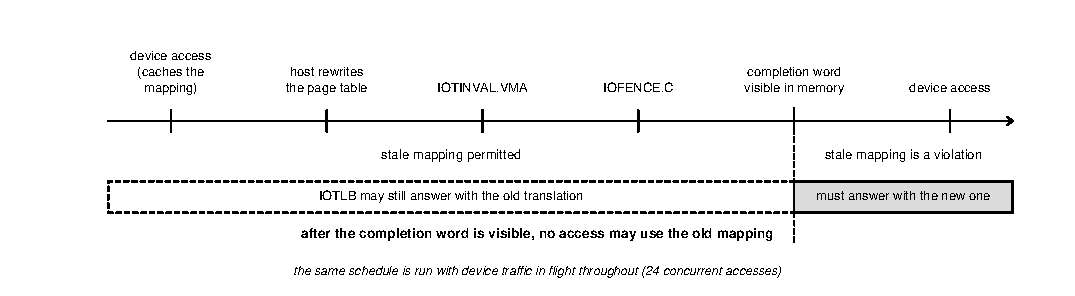
\includegraphics[width=\textwidth]{figures/figB1_ordering.pdf}
\caption{The schedule underlying P5. Before the fence completion is visible the
IOMMU may answer from its cache; after it, it may not. The same schedule is run
with device traffic in flight throughout.}
\label{fig:order}
\end{figure*}

We state five properties. Each is decided by observing the address that leaves
the IOMMU's completion port for a device transaction, so each is testable on any
implementation without internal visibility.

\textbf{P1 (staleness permitted).} If a page-table entry is modified and no
invalidation is issued, a transaction to that page may be answered with the old
translation. This is the control: it confirms that the cache is active and that
the later properties are not vacuously satisfied by an implementation that
simply never caches.

\textbf{P2 (effectiveness).} After an unscoped invalidation, a transaction to
the affected page must be answered with the new translation, and the IOMMU must
have re-read the page tables to obtain it.

\textbf{P3 (scope precision).} After an invalidation scoped to one address, a
transaction to that address must be answered with the new translation.

\textbf{P4 (scope containment).} The same scoped invalidation must not disturb
other cached translations: a transaction to a different cached page must still
be answered from the cache. P3 and P4 together pin the scope from both sides; an
implementation that ignores scope and flushes everything satisfies P3 and fails
P4, and one that ignores the command satisfies P4 and fails P3.

\textbf{P5 (completion ordering).} Once the fence's completion word is visible
in memory, no subsequent transaction may be answered with a translation removed
by a command preceding the fence (Fig.~\ref{fig:order}).

\textbf{P5$'$ (completion ordering under load).} P5 must hold when device
transactions are in flight across the whole sequence, not only when the device
is quiescent while software invalidates.

\section{Method}
We realise the properties against the open RISC-V IOMMU IP published by
Zero-Day Labs~\cite{rviommu}, using a Verilator environment that drives the
device's four AXI interfaces, serves its implicit page-table and command-queue
accesses from a memory image, and observes translated addresses on the
completion port. The environment and its construction are described
separately~\cite{companion}; what matters here is that the testbench owns the
memory image, so it can modify a page-table entry between two device
transactions and can poll for the fence completion word directly.

Each property becomes a schedule. For P1: map a page, access it so the
translation is cached, rewrite the leaf entry to a different physical page,
access it again, and require the old address. For P2: repeat, but enqueue an
unscoped \cmd{IOTINVAL.VMA} first, and require both the new address and
evidence that a walk occurred. For P3 and P4: cache two pages, rewrite both
entries, invalidate only the first, and require the first to be refreshed and the
second to be unchanged. For P5: rewrite an entry, enqueue the invalidation
followed by \cmd{IOFENCE.C} with a completion address, poll the image for the
completion word, and only then issue the transaction.

Three details make these schedules trustworthy, and each was a correction to an
earlier version of the environment.

First, the page-table rewrite must not be visible to the IOMMU as anything but a
memory change. The testbench writes the new leaf entry directly into its memory
image rather than through any hardware path, so a cached translation can only be
refreshed by the IOMMU re-reading the entry.

Second, ``the translation was refreshed'' must be distinguished from ``the
translation happened to be right.'' The environment counts the implicit accesses
the IOMMU issues on its data-structure port, so P2 can require both the new
address on the completion port and evidence that a walk occurred; an
implementation that returned the correct address without re-reading memory would
be caching something it should not.

Third, the fence completion must be observed the way software observes it. The
testbench polls its memory image for the completion word at the address supplied
in the command, exactly as a driver polls the completion location, rather than
watching an internal signal. This matters because the property is about what is
visible to software, and an internal ``invalidation done'' signal may assert
earlier than the word appears.

P5$'$ uses two concurrent processes. One issues a stream of twenty-four
transactions to the affected page with a short gap between them. The other
waits, enqueues the invalidation and fence, and sets a flag when the completion
word appears. Every transaction the first process completes after that flag is
set is checked against the new translation; transactions completed before it are
unconstrained. The schedule is arranged so that a useful number of transactions
fall on each side of the boundary---if all of them landed before the fence the
test would be vacuous---and the test records the split, so a run in which too
few transactions were post-fence is visible rather than silently weak.

\section{Results}

\begin{table}[!t]
\caption{Ordering properties on the implementation under test}
\label{tab:props}
\centering\footnotesize
\begin{tabular}{llc}
\toprule
 & Property & Result \\
\midrule
P1  & staleness permitted before invalidation & holds \\
P2  & invalidation is effective (forces re-walk) & holds \\
P3  & scoped invalidation refreshes the named page & holds \\
P4  & scoped invalidation leaves other pages cached & holds \\
P5  & no stale translation after fence completion & holds \\
P5$'$ & P5 under twenty-four concurrent transactions & holds \\
\bottomrule
\end{tabular}
\end{table}

Table~\ref{tab:props} summarises. All six hold. Thirteen of the fifty-six checks
in the wider suite belong to this family.

Quantitatively: under P2 the invalidated access re-reads the page tables, which
the environment confirms by counting the implicit accesses the IOMMU issues.
Under P4 the untouched page is still answered from the cache with its original
translation, so the scope is neither too wide nor ignored. Under a variant of P2
that caches four pages---filling the IOTLB in the configuration under test---and
then invalidates all of them, all four are refreshed. Under P5 the fence
completion word appears twelve cycles after the command is enqueued, and the
subsequent transaction uses the new translation. Under P5$'$, twenty of the
twenty-four transactions complete after the fence completion becomes visible,
and none of them uses the stale translation (Fig.~\ref{fig:conc}, upper row).

\begin{figure*}[!t]
\centering
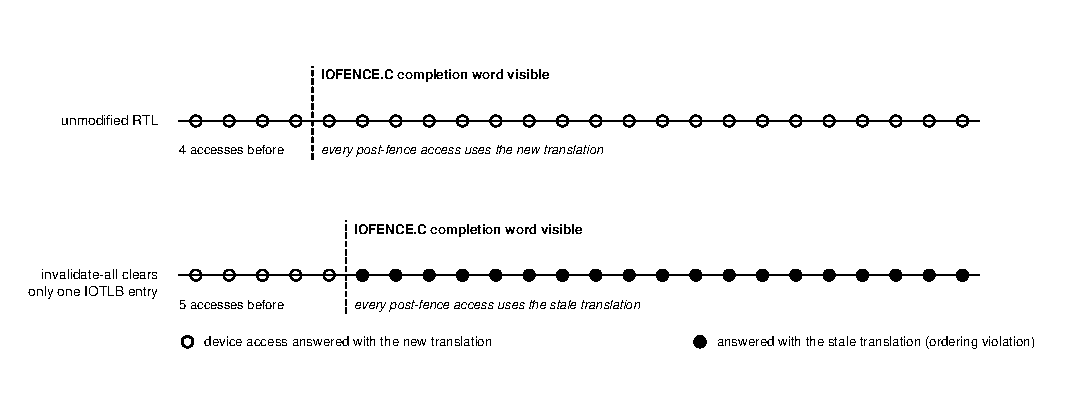
\includegraphics[width=\textwidth]{figures/figB2_concurrent.pdf}
\caption{P5$'$ on the unmodified design and on a design with a partial-flush
defect injected. Each marker is one device transaction. The property constrains
only the transactions to the right of the dashed line. The defect is invisible
before the fence and total after it.}
\label{fig:conc}
\end{figure*}

The last figure is worth reading as a statement about the property rather than
about the design. To the left of the dashed line the two rows are
indistinguishable, and correctly so: nothing is being claimed there. Everything
the property says is to the right of it, and that is exactly where the two rows
separate completely.

\section{Do the Tests Discriminate?}
A suite in which everything passes is worth little unless it can be shown to
fail when it should. We injected two invalidation defects into the RTL, each a
single scripted edit, rebuilt and reran.

The first makes invalidation ineffective: the IOTLB entry is not cleared when a
matching invalidation arrives. Six checks fail, P2 among them.

The second is subtler and is the reason P2 was extended to the multi-page case.
It makes an unscoped invalidation clear only the first IOTLB entry, leaving the
rest stale---the shape of a real partial-flush bug. It is detected by four
checks. A suite that invalidated and rechecked a single page would have passed
this defect, because the single page it checked would be the entry that was
cleared.

\begin{table}[!t]
\caption{Injected invalidation defects}
\label{tab:mut}
\centering\footnotesize
\begin{tabular}{@{}p{5.2cm}cl@{}}
\toprule
Defect & \shortstack{Checks\\failed} & \shortstack{Caught\\by} \\
\midrule
IOTLB entry not cleared on a matching invalidation & 6 & P2 \\
Unscoped invalidation clears only the first IOTLB entry & 4 & P2$^{*}$ \\
\bottomrule
\end{tabular}
\\[2pt]
\footnotesize $^{*}$only by the multi-page form of P2.
\end{table}

Table~\ref{tab:mut} records both. Under the partial-flush defect, P5$'$ reports
nineteen stale translations out of nineteen post-fence transactions
(Fig.~\ref{fig:conc}, lower row): once the surviving entry is the one the device
is using, every transaction after the fence is wrong. That is what the failure
looks like in hardware, and it is the reason we consider the concurrent variant
worth the extra machinery---it is the test that turns a single wrong address
into an unmistakable pattern.

We draw two methodological points from this. The first is that the multi-page
form of P2 is not redundancy; it is the only thing separating a suite that
catches partial-flush defects from one that does not, and single-page
invalidation tests are the natural thing to write. The second is that both
defects are single-line edits that leave the design fully functional---it
translates, it walks, it faults correctly---which is a fair model of how such a
bug reaches silicon. Neither is caught by any test outside this property family.

\section{The Guarantee Is Incidental}
The implementation satisfies P5, but the reason deserves scrutiny. Its command
handler implements \cmd{IOFENCE.C} by writing the completion word when the
command is processed; it does not wait for preceding commands to retire. The
source states the reasoning directly, and anticipates the problem:

\begin{quote}\footnotesize
``I think this command makes sense when implementing ATS commands, or any other
command that could take several cycles to execute. [\ldots] Since all
implemented commands in this version are executed immediately, there's no need
to wait for now.''
\end{quote}

\noindent The comment is right on both counts. The fence is for long-latency
commands, and there are none yet.

That argument is sound for the current feature set and unsound as a design
property. \cmd{IOFENCE.C} exists precisely to order commands whose effects
are not immediate. The specification's ATS invalidation commands, which this
implementation does not provide, require a round trip to a device and are
exactly the long-latency case the fence is for; the same applies to any future
command whose effect is pipelined rather than combinational. When such a command
is added, P5 will no longer follow from the structure of the design, and nothing
in the current implementation will notice: the fence will keep completing
immediately and the tests will keep passing until a command is slow enough for
the window to open. The implementation also marks the fence's
predecessor-read and predecessor-write bits as unimplemented.

This is the practical value we would claim for the property family. P5 as tested
is satisfied today. Kept in a regression suite, it becomes a guard on the
assumption that makes it true, and it will fail on the day that assumption stops
holding.

\section{Applying the Properties Elsewhere}
Nothing in P1--P5$'$ is specific to RISC-V. Each is stated in terms of three
capabilities that any IOMMU offers in some form: a way to cause a translation to
be cached, a way to invalidate it, and a way to learn that the invalidation has
taken effect. An ARM SMMU expresses the second and third as \texttt{TLBI}
commands followed by a synchronisation command whose completion is polled in a
consumer register; an Intel VT-d unit expresses them as invalidation descriptors
followed by an invalidation-wait descriptor that writes a status word to memory,
which is close enough to \cmd{IOFENCE.C} that the P5 schedule transfers
almost unchanged. The scoping distinctions behind P3 and P4 map onto those
architectures' domain- and address-selective invalidations.

What must be rebuilt for each target is the observation path: the properties are
decided by watching the physical address an IOMMU emits, so they need an
environment that can see that port and that owns the memory image the IOMMU
walks. That is the bulk of the work, and it is work a verification team doing
anything else with the design has already done. Added to an existing
environment, the property family is a few hundred lines.

Two things would have to be reconsidered for a design with a deeper pipeline
than the one we tested. P5$'$ assumes that a transaction observed at the
completion port after the fence word appeared was in fact decided after it;
in a design that speculates on translations or that reorders completions, that
inference needs an additional argument or an internal probe. And a design with
multiple independent translation caches---per-device or per-context---needs P4
restated over each of them, since an invalidation that reaches one cache and not
another is precisely the defect the property is meant to catch.

\section{Limitations}
This is a study of one implementation, and a negative result in the sense that
no violation was found. The properties are stated operationally rather than
formally; we do not claim they are complete, and a formal treatment in the style
of the transistency work would likely yield more. Only first-stage invalidation
is exercised: second-stage (\cmd{IOTINVAL.GVMA}) and directory-cache
(\cmd{IODIR}) invalidation are not, nor is invalidation scoped by
address-space or virtual-machine identifier, nor are ATS invalidations, which
the implementation does not provide. Concurrency is exercised with a single
device stream; multiple devices with distinct identifiers invalidating and
translating simultaneously would be a stronger test. All results come from
simulation of one implementation with one simulator, at one configuration of
IOTLB and directory-cache sizes; the multi-page form of P2 uses four pages
because that fills the cache in this configuration, and the number would have to
be re-chosen for a larger one. Finally, fault injection measures whether the
tests catch the defects we thought to inject, which is evidence that they
discriminate but not a bound on what they would miss.

\section{Conclusion}
The ordering obligation an IOMMU owes to an operating system's unmap path is
testable, cheaply, against RTL, and it is not covered by the CPU-side work on
translation-aware memory ordering. Five properties, expressed as schedules over
the command interface and decided by watching the completion port, are enough to
pin the boundary from both sides---requiring staleness to end after the fence,
and requiring scoped invalidation not to over-reach. An open RISC-V IOMMU
satisfies all of them, including under concurrent traffic, and two injected
invalidation defects are caught. The implementation's fence, however, does not
wait for preceding commands; its compliance rests on every implemented command
being immediate, which is a fact about today's feature set rather than a
guarantee of the design.

The result we would most like to be acted on is the cheapest one. These are six
tests. They run in seconds, they need no formal model and no proprietary tools,
and they belong in the regression suite of any IOMMU under development---not
because they are likely to fail today, but because the assumption that makes
them pass is the kind that is quietly invalidated by a feature added two years
later by someone who never read the comment explaining why the fence did not
need to wait.

\section*{Artifact Availability}
The tests, the environment they run in, and the fault-injection harness are
released under a permissive licence and run with open tools.

\begin{thebibliography}{9}
\bibitem{coatcheck} D.~Lustig, G.~Sethi, M.~Martonosi, and A.~Bhattacharjee,
``COATCheck: Verifying memory ordering at the hardware--OS interface,'' in
\emph{ASPLOS}, 2016.
\bibitem{transform} N.~Manerkar, D.~Lustig, M.~Martonosi, and A.~Bhattacharjee,
``TransForm: Formally specifying transistency models and synthesizing enhanced
litmus tests,'' in \emph{ISCA}, 2018.
\bibitem{rtlcheck} Y.~A.~Manerkar, D.~Lustig, M.~Martonosi, and M.~Pellauer,
``RTLCheck: Verifying the memory consistency of RTL designs,'' in \emph{MICRO},
2017.
\bibitem{realitycheck} Y.~A.~Manerkar, D.~Lustig, and M.~Martonosi,
``RealityCheck: Bringing modularity, hierarchy and abstraction to automated
microarchitectural memory consistency verification,'' arXiv:2003.04892, 2020.
\bibitem{qed} ``QED: Scalable verification of hardware memory consistency,''
arXiv:2404.03113, 2024.
\bibitem{thunderclap} A.~T.~Markettos, C.~Rothwell, B.~F.~Gutstein, A.~Pearce,
P.~G.~Neumann, S.~W.~Moore, and R.~N.~M.~Watson, ``Thunderclap: Exploring
vulnerabilities in operating system IOMMU protection via DMA from untrustworthy
peripherals,'' in \emph{NDSS}, 2019.
\bibitem{iotlb} N.~Amit, M.~Ben-Yehuda, and B.-A.~Yassour, ``IOMMU: Strategies
for mitigating the IOTLB bottleneck,'' in \emph{Workshop on Interaction between
Operating Systems and Computer Architecture (WIOSCA)}, 2010.
\bibitem{litmusriscv} ``litmus-tests-riscv: RISC-V architecture concurrency
model litmus tests.'' [Online]. Available:
\url{https://github.com/litmus-tests/litmus-tests-riscv}
\bibitem{rviommu} Zero-Day Labs, ``RISC-V IOMMU IP,'' commit \texttt{18ad30a}.
[Online]. Available: \url{https://github.com/zero-day-labs/riscv-iommu}
\bibitem{companion} M.~Timbadiya, ``Verifying the RISC-V IOMMU: an open
verification environment and a fault-injection evaluation,'' companion article.
\end{thebibliography}

\end{document}
